% !TEX encoding = UTF-8
% !TEX TS-program = pdflatex
% !TEX root = ../tesi.tex

%**************************************************************
\chapter{Appendice A}
%**************************************************************

\hypertarget{integrazione-di-monokee-single-sign-on-oidc-tramite-freeipa}{%
\section{Integrazione di Monokee Single Sign-On (OIDC) tramite
FreeIPA}\label{integrazione-di-monokee-single-sign-on-oidc-tramite-freeipa}}


% ================== INDICE =============================
\hypertarget{indice}{%
\subsection{Indice}\label{indice}}

\begin{itemize}
\tightlist
\item
  \protect\hyperlink{integrazione-di-monokee-single-sign-on-oidc-tramite-freeipa}{Integrazione
  di Monokee Single Sign-On (OIDC) tramite FreeIPA}

  \begin{itemize}
  \tightlist
  \item
    \protect\hyperlink{indice}{Indice}
  \item
    \protect\hyperlink{introduzione-guida}{Introduzione}
  \item
    \protect\hyperlink{installazione-di-freeipa}{Installazione di
    FreeIPA}

    \begin{itemize}
    \tightlist
    \item
      \protect\hyperlink{requisiti-di-sistema}{Requisiti di sistema}
    \item
      \protect\hyperlink{installazione}{Installazione}
    \item
      \protect\hyperlink{accesso-a-freeipa}{Accesso a FreeIPA}
    \end{itemize}
  \item
    \protect\hyperlink{setup-monokee}{Setup Monokee}

    \begin{itemize}
    \tightlist
    \item
      \protect\hyperlink{app-oauth}{App OAuth}
    \item
      \protect\hyperlink{openid-connect-provider}{OpenID Connect
      Provider}
    \end{itemize}
  \item
    \protect\hyperlink{setup-idp-freeipa}{Setup IdP FreeIPA}

    \begin{itemize}
    \tightlist
    \item
    \protect\hyperlink{setup-identity-provider-server}{Setup Identity
    Provider Server}
    \item
    \protect\hyperlink{setup-utenti}{Setup Utenti}
  \end{itemize}
  \item
  \protect\hyperlink{autenticazione-via-cli}{Autenticazione via CLI}
\end{itemize}
\end{itemize}
% =============================================================


\hypertarget{introduzione-guida}{%
\subsection{Introduzione}\label{introduzione-guida}}
Il seguente documento illustra il procedimento per disporre un ambiente di Single Sign-On che utilizzi Monokee con OpenID Connect come external Identity Provider di FreeIPA.

\hypertarget{installazione-di-freeipa}{%
\subsection{Installazione di FreeIPA}\label{installazione-di-freeipa}}

\hypertarget{requisiti-di-sistema}{%
\subsubsection{Requisiti di sistema}\label{requisiti-di-sistema}}

Per il server su cui installare FreeIPA è consigliata una macchina con
CentOS Stream 9.

È consigliabile anche lanciare i seguenti comandi per installare
pacchetti utili: EPEL (Extra Packages for Enterprise Linux) è un insieme
di pacchetti di Fedora non presenti nativamente su sistemi RHEL,
\emph{bind-utils} contiene dei comandi per ottenere facilmente
informazioni riguardanti i DNS, Vim è un editor di testo.

\begin{verbatim}
sudo yum -y install epel-release
sudo yum -y update
sudo yum install bind-utils vim
\end{verbatim}

\hypertarget{installazione}{%
\subsubsection{Installazione}\label{installazione}}

Lanciare il seguente comando per scaricare il pacchetto di FreeIPA.

\begin{verbatim}
sudo yum -y install ipa-server
\end{verbatim}

In questa guida utilizzeremo FQDN, invece che DNS, per comodità. È
sufficiente modificare il file \emph{/etc/hosts} aggiungendo l'indirizzo
IP della macchina su cui si sta effettuando l'installazione.

\begin{verbatim}
sudo vim /etc/hosts
10.0.3.190  ipa.server.com
\end{verbatim}

Configurare l'hostname con lo stesso nome utilizzato nel file
\emph{/etc/hosts}.

\begin{verbatim}
sudo hostnamectl set-hostname ipa.server.com
\end{verbatim}

Lanciare il comando di installazione.

\begin{verbatim}
sudo ipa-server-install
\end{verbatim}

Appariranno una serie di domande a schermo: è sufficiente premere
\emph{Invio} a tutte tranne che all'ultima, di conferma, a cui bisogna
rispondere in modo affermativo. Inoltre, verrà chiesto di inserire e
confermare delle password. Dopo qualche minuto dovrebbe apparire un
messaggio di riuscita installazione.

\begin{verbatim}
Continue to configure the system with these values? [no]: yes

The following operations may take some minutes to complete.
Please wait until the prompt is returned.

Configuring NTP daemon (ntpd)
  [1/4]: stopping ntpd
  [2/4]: writing configuration
  [3/4]: configuring ntpd to start on boot
  [4/4]: starting ntpd
Done configuring NTP daemon (ntpd).
Configuring directory server (dirsrv). Estimated time: 30 seconds
.....
Client configuration complete.
The ipa-client-install command was successful

==============================================================================
Setup complete

Next steps:
    1. You must make sure these network ports are open:
        TCP Ports:
          * 80, 443: HTTP/HTTPS
          * 389, 636: LDAP/LDAPS
          * 88, 464: kerberos
        UDP Ports:
          * 88, 464: kerberos
          * 123: ntp

    2. You can now obtain a kerberos ticket using the command: 'kinit admin'
       This ticket will allow you to use the IPA tools (e.g., ipa user-add)
       and the web user interface.

Be sure to back up the CA certificates stored in /root/cacert.p12
These files are required to create replicas. The password for these
files is the Directory Manager password
...
\end{verbatim}

È possibile che debbano essere aperte alcune porte in presenza di un
firewall attivo, si consiglia, dunque, di lanciare i seguenti comandi.
Se il firewall non è attivo, si consiglia comunque di attivarlo e
lanciare i comandi seguenti.

\begin{verbatim}
sudo firewall-cmd --add-service={dns,freeipa-ldap,freeipa-ldaps} --permanent
sudo firewall-cmd --reload
\end{verbatim}

\hypertarget{accesso-a-freeipa}{%
\subsubsection{Accesso a FreeIPA}\label{accesso-a-freeipa}}

È possibile accedere a FreeIPA da CLI, richiedendo un ticket Kerberos
con il comando \texttt{kinit\ admin} oppure dall'interfaccia web,
all'indirizzo uguale all'hostname che si è utilizzato
(https://ipa.server.com/), inserendo come username \emph{admin}; in
entrambi i casi la password corrisponde a quella scelta durante il
processo di installazione.

\begin{figure}[!h] 
  \centering 
  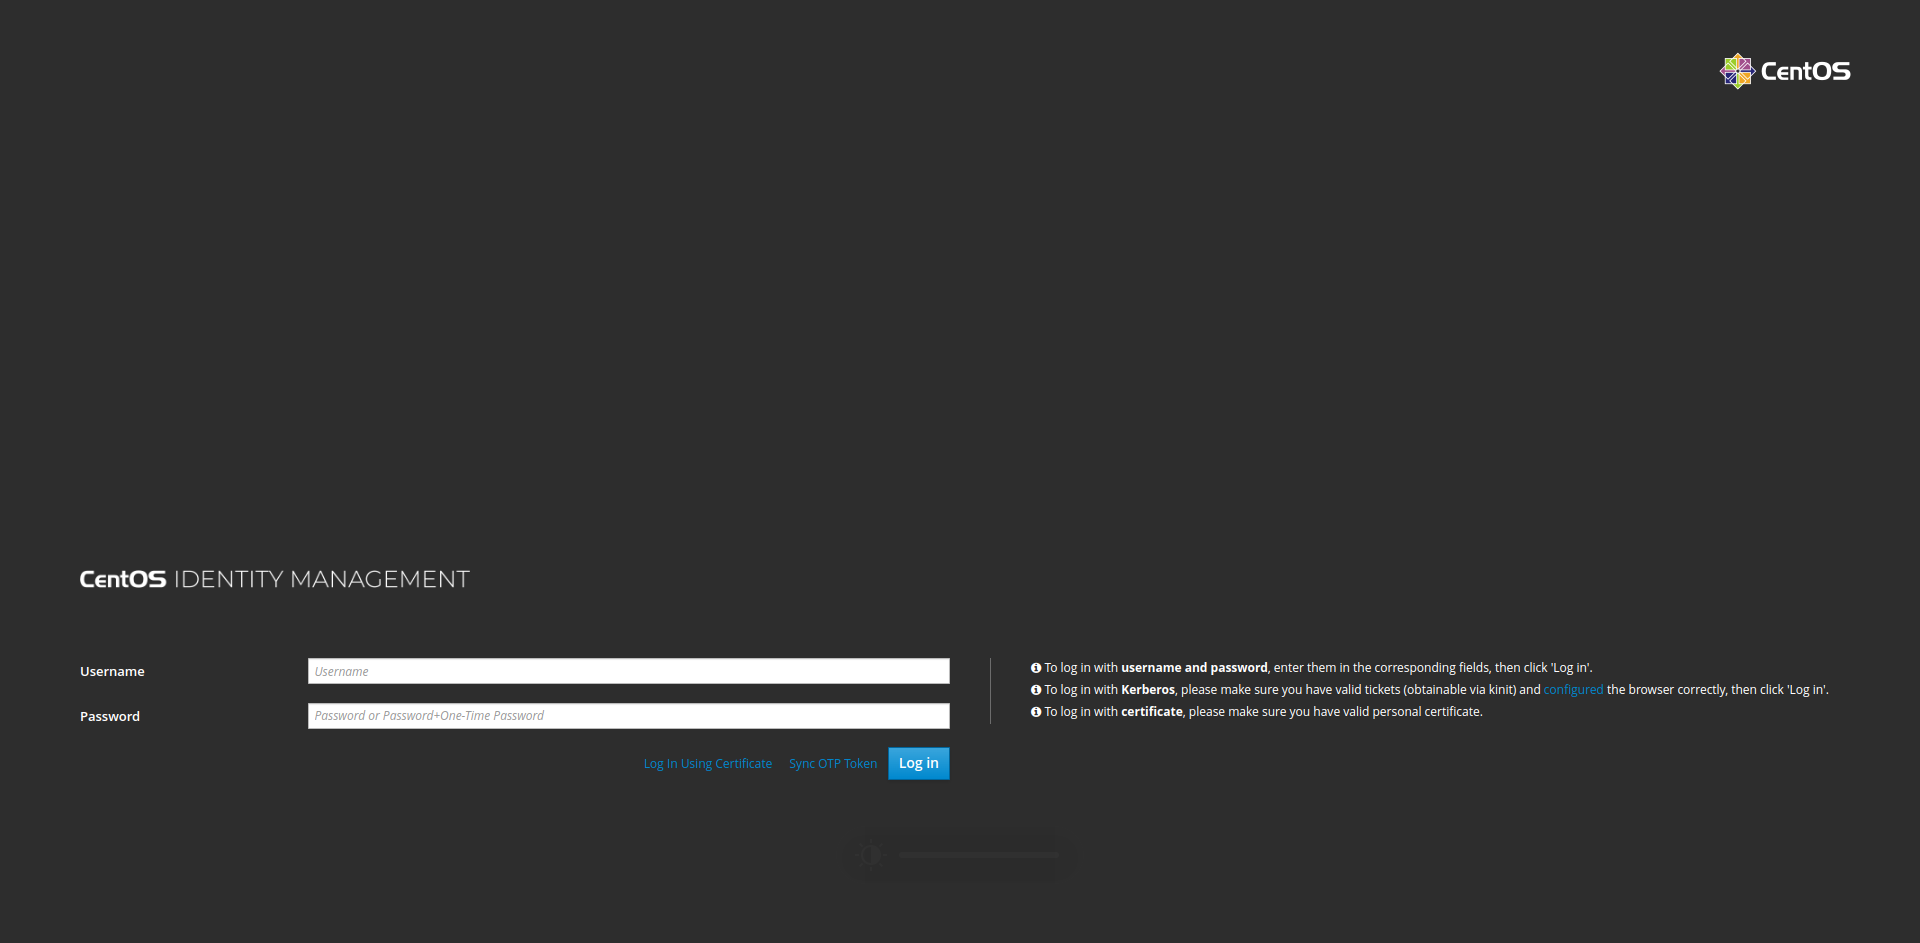
\includegraphics[width=\columnwidth]{appendici/ipa-login} 
  \caption{Vista schermata di login FreeIPA}
\end{figure}

\hypertarget{setup-monokee}{%
\subsection{Setup Monokee}\label{setup-monokee}}

\hypertarget{app-oauth}{%
\subsubsection{App OAuth}\label{app-oauth}}

Su \url{test.monokee.com} andare nella sezione \emph{Applications},
creare una nuova applicazione OAuth.

\begin{figure}[!h] 
  \centering 
  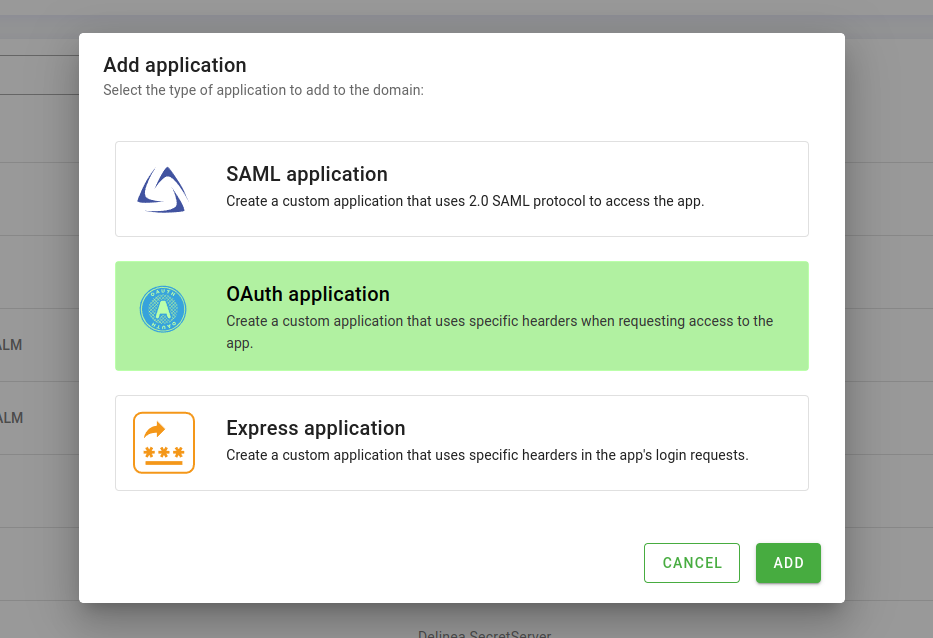
\includegraphics[width=\columnwidth]{appendici/monokee-oauth-app} 
  \caption{Vista nuova app OAuth2 da Monokee}
\end{figure}


In \emph{Application assets}, aggiungere gli utenti (e/o i gruppi di
utenti) ai quali si vuole consentire l'accesso sia nella sezione
\emph{Users} (e/o \emph{Groups}) che nella relativa sezione in
\emph{Scopes}.

\begin{figure}[!h] 
  \centering 
  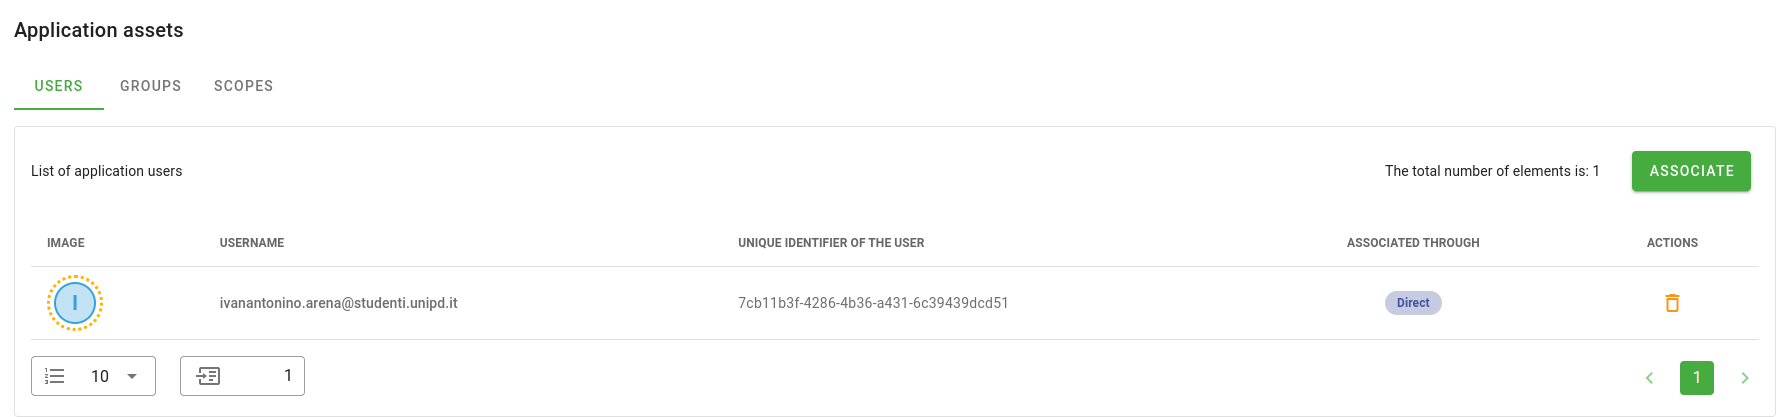
\includegraphics[width=\columnwidth]{appendici/monokee-oauth-users} 
  \caption{Vista OAuth users}
\end{figure}


Andare sull'icona della matita per modificare l'applicazione e cliccare
su \emph{Next} per passare alle impostazioni del client. Qui scegliere
un \emph{Client ID} ed un \emph{Client Secret} (quest'ultimo è possibile
anche lasciarlo vuoto) ed impostare gli altri valori come da figura.

\begin{figure}[!h] 
  \centering 
  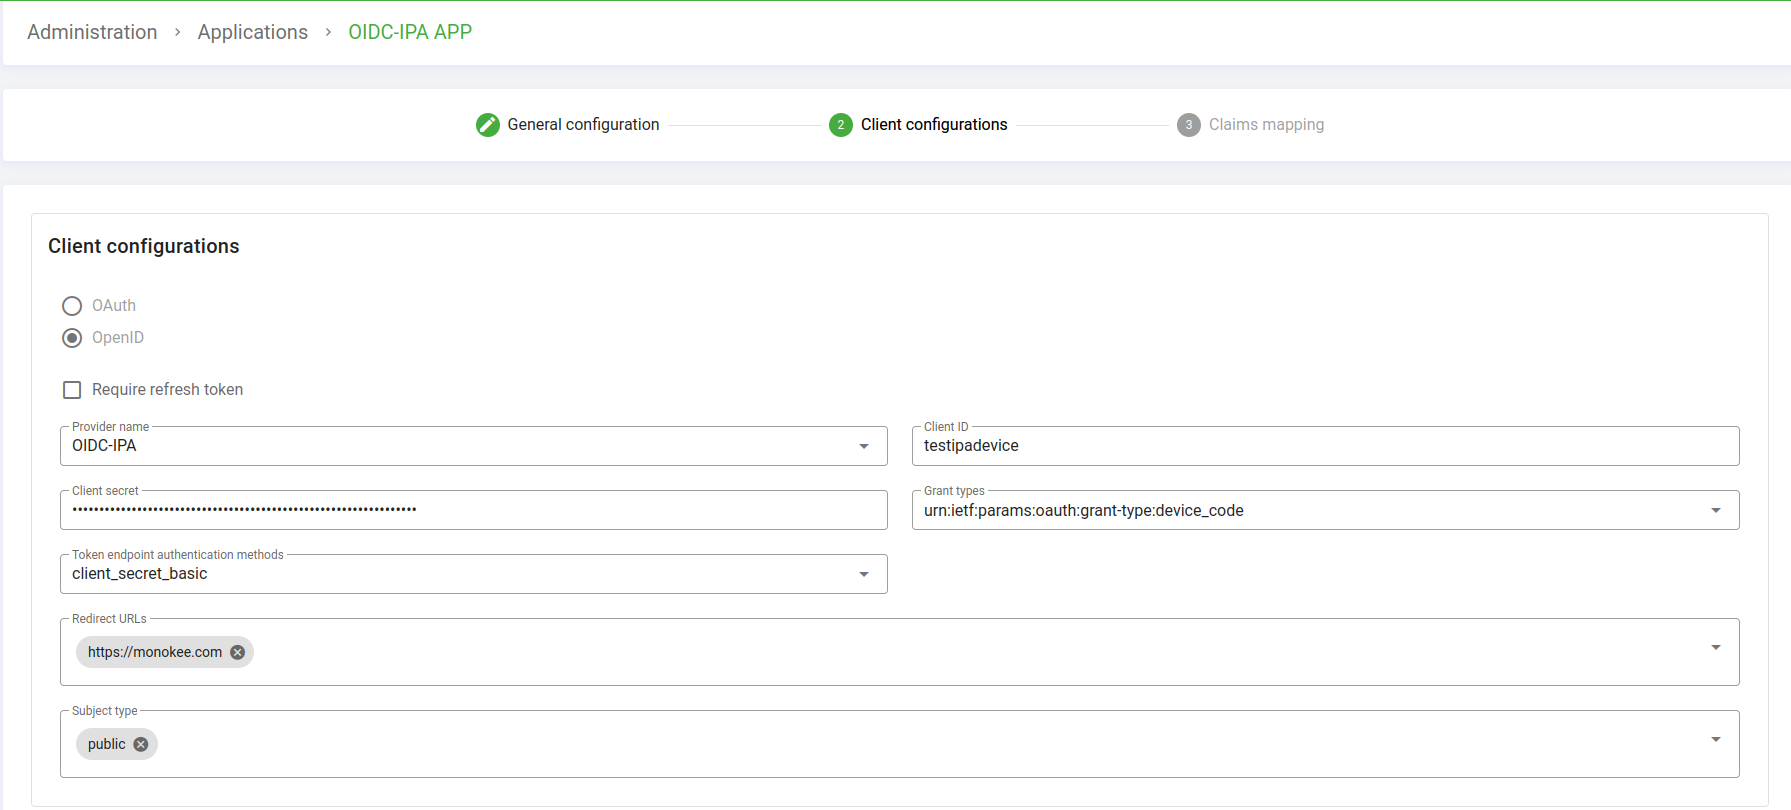
\includegraphics[width=\columnwidth]{appendici/monokee-oauth-client} 
  \caption{Vista OAuth client configuration da Monokee}
\end{figure}

\begin{figure}[!h] 
  \centering 
  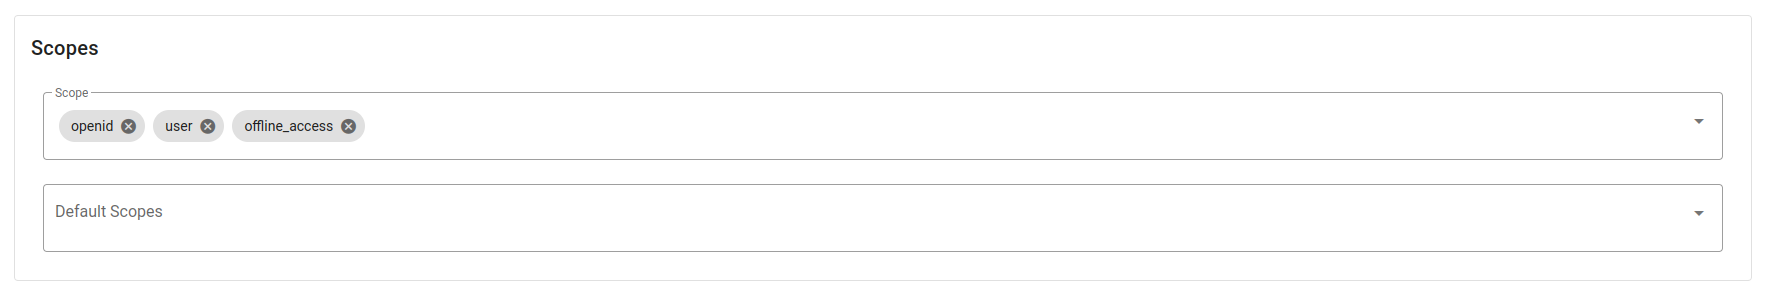
\includegraphics[width=\columnwidth]{appendici/monokee-oauth-client-scopes} 
  \caption{Vista client scopes}
\end{figure}


Cliccare nuovamente su \emph{Next} ed impostare i valori della pagina
come da figura.

\begin{figure}[!h] 
  \centering 
  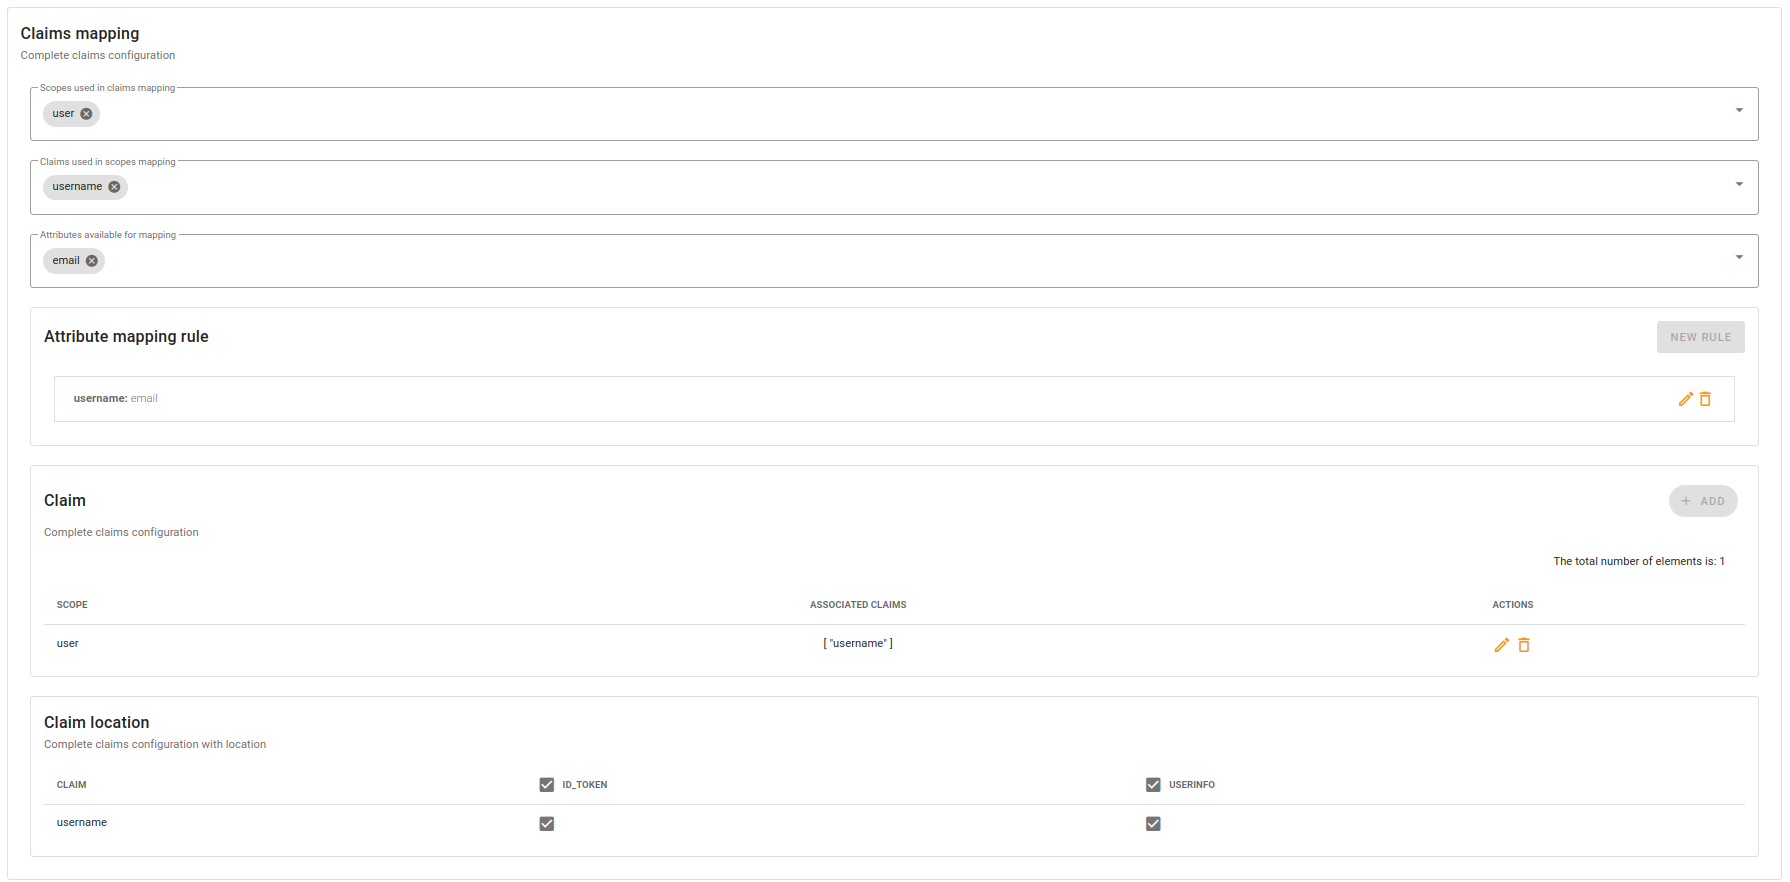
\includegraphics[width=\columnwidth]{appendici/monokee-oauth-mapping} 
  \caption{Vista application assets}
\end{figure}


\hypertarget{openid-connect-provider}{%
\subsubsection{OpenID Connect Provider}\label{openid-connect-provider}}

Spostarsi nella sezione \emph{OAuth Providers} ed aggiungere un nuovo
OpenID Provider nell'apposita vista.

\begin{figure}[!h] 
  \centering 
  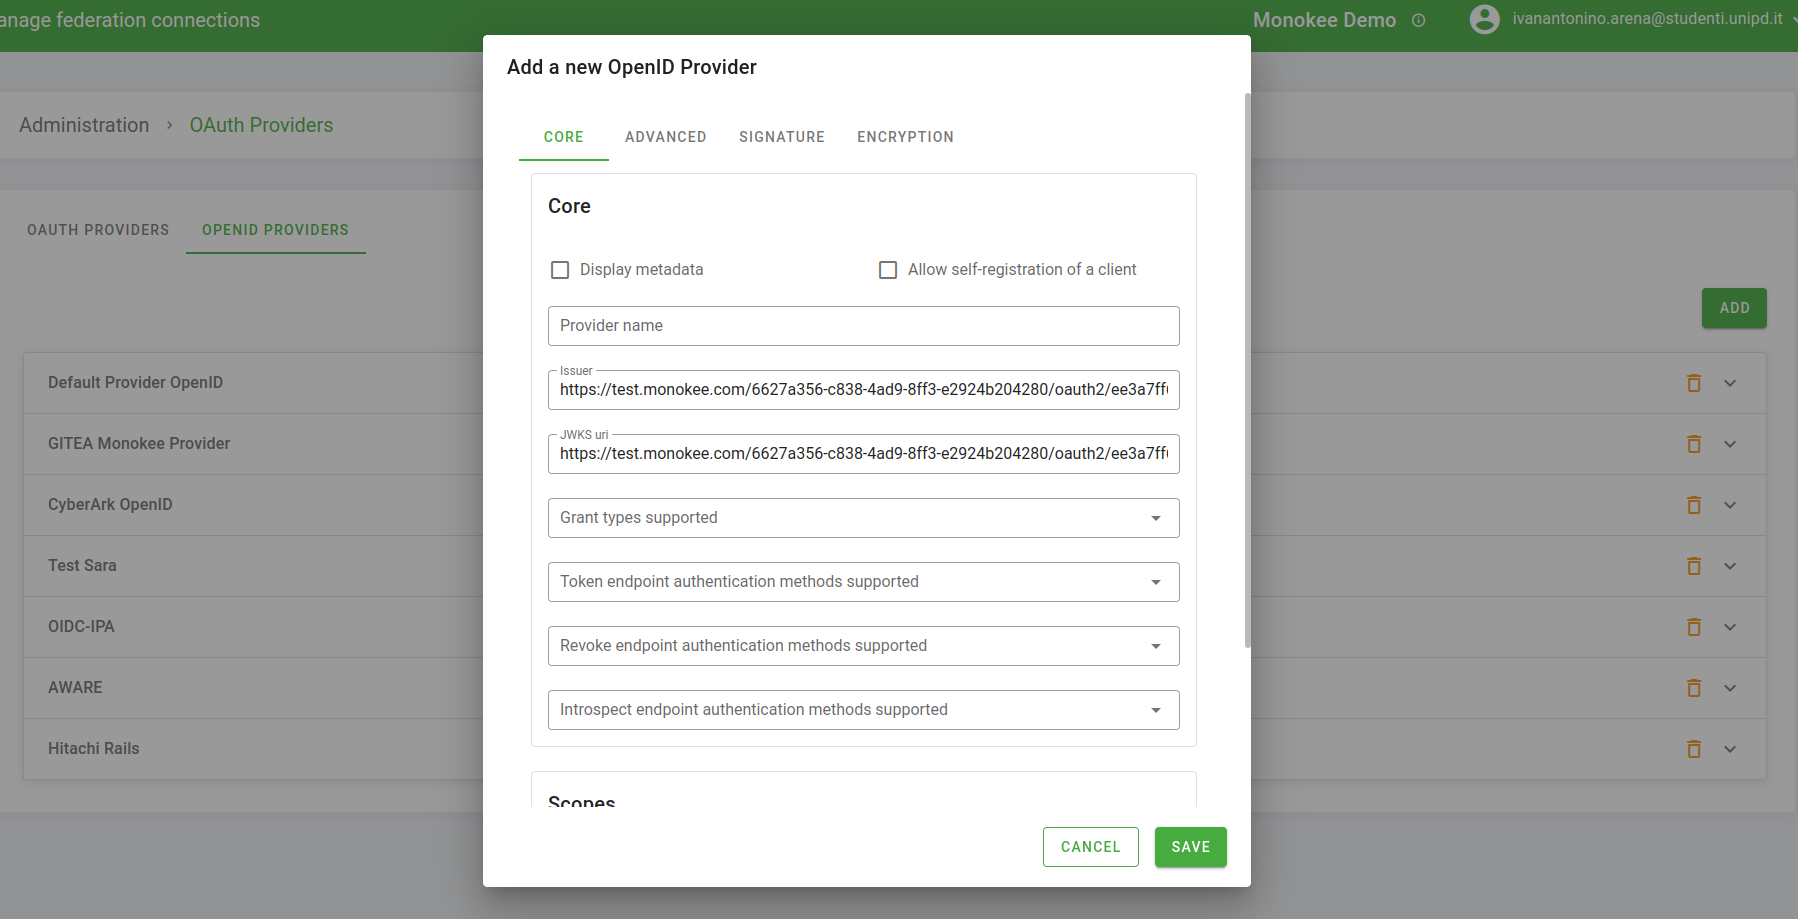
\includegraphics[width=\columnwidth]{appendici/monokee-oidc} 
  \caption{Vista nuovo OpenID provider da Monokee}
\end{figure}


Spuntare l'opzione \emph{Display metadata}, scegliere un nome per il
provider ed inserire i valori come da figura.

\begin{figure}[!h] 
  \centering 
  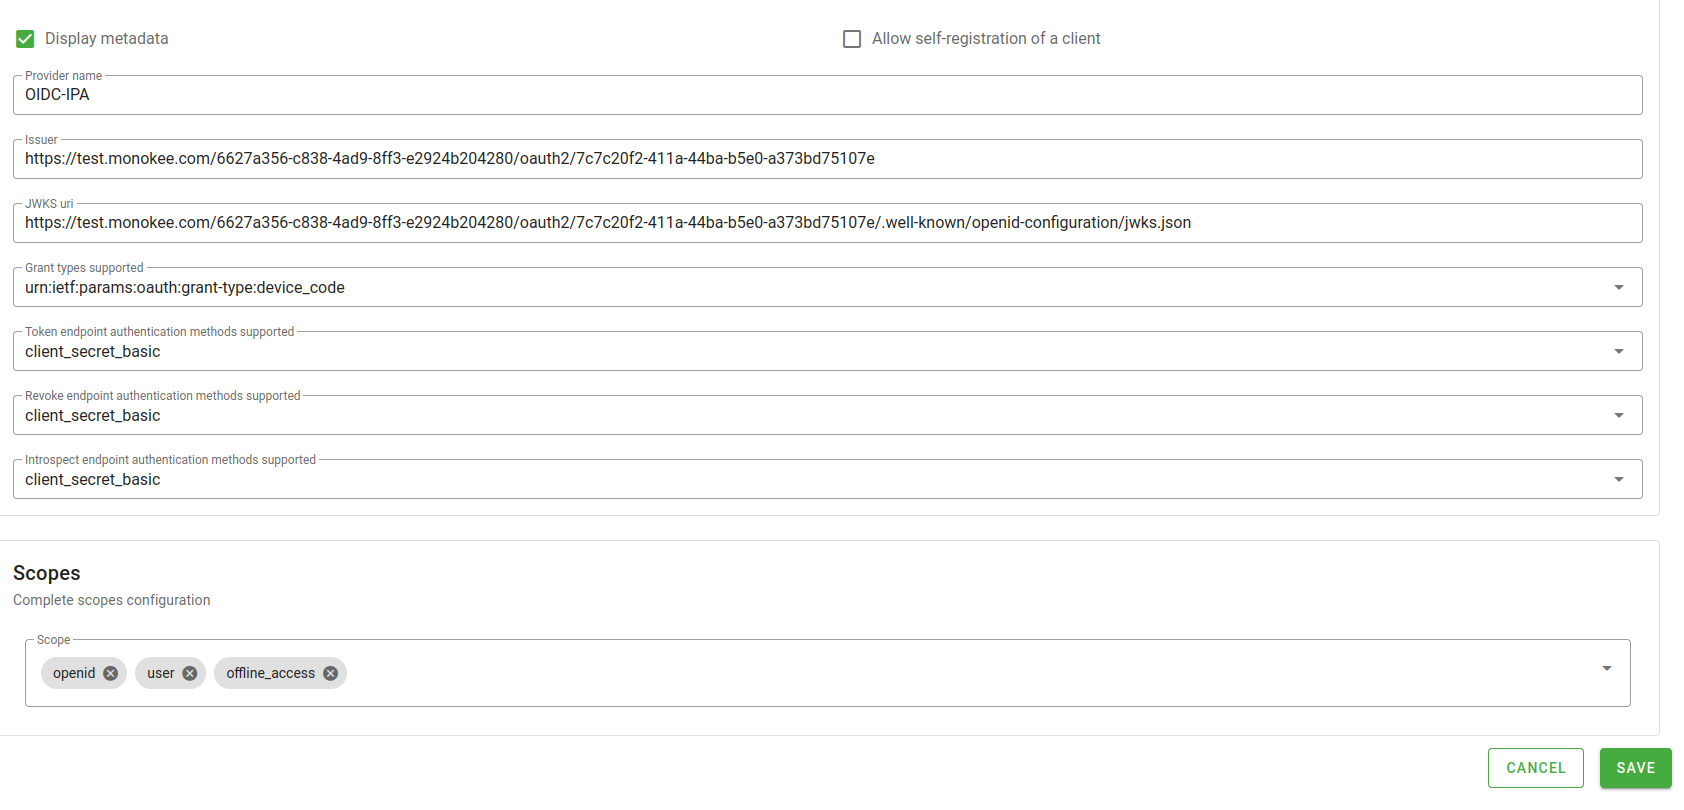
\includegraphics[width=\columnwidth]{appendici/monokee-oidc-provider} 
  \caption{Valori OpenID provider}
\end{figure}


Spostarsi nella sezione \emph{Advanced} ed impostare i valori come da
figura.

\begin{figure}[!h] 
  \centering 
  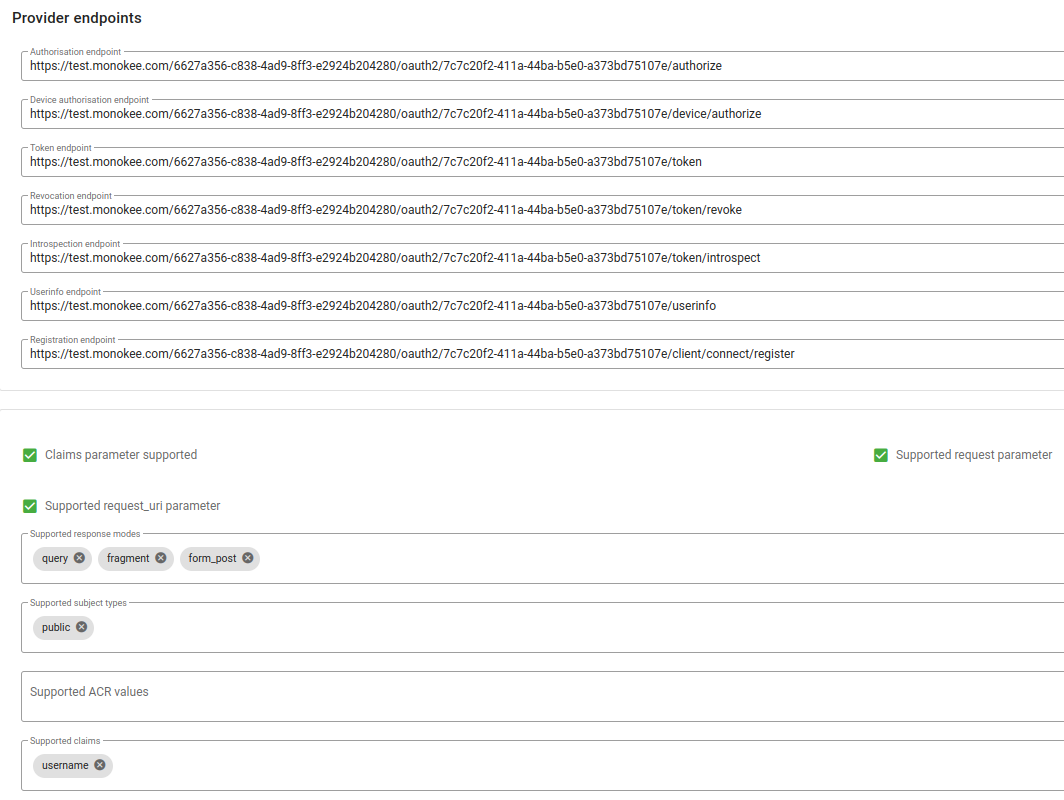
\includegraphics[width=\columnwidth]{appendici/monokee-oidc-advanced} 
  \caption{Valori OpenID provider Advanceds}
\end{figure}


\hypertarget{setup-idp-freeipa}{%
\subsection{Setup IdP FreeIPA}\label{setup-idp-freeipa}}

\emph{NB: è possibile effettuare le seguenti operazioni anche da
terminale con degli specifici comandi, tuttavia, per comodità, viene
mostrato il procedimento da web UI.} \#\#\# Setup Identity Provider
Server

Autenticarsi sulla web UI di FreeIPA e spostarsi nella sezione
\emph{Authentication} \textgreater{} \emph{Identity Provider servers},
cliccare su \emph{Add} per creare un nuovo Identity Provider, scegliere
un nome e compilare i campi con i rispettivi dati ed endpoint
dell'applicazione OAuth e dell'OpenID Provider impostati
precedentemente.

\begin{figure}[!h] 
  \centering 
  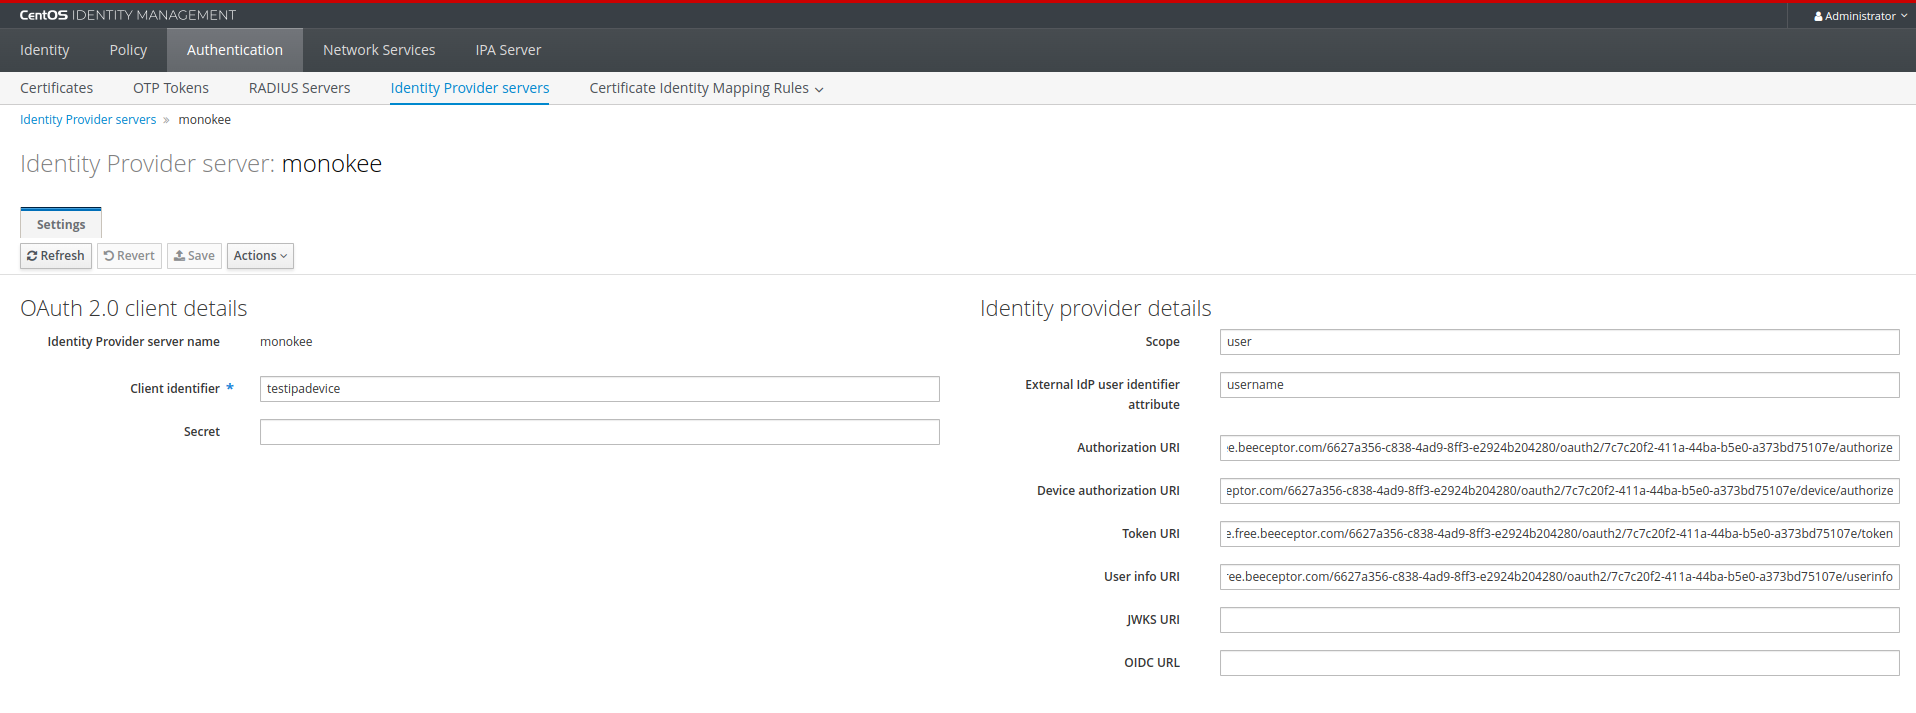
\includegraphics[width=\columnwidth]{appendici/ipa-idp} 
  \caption{Valori Identity Provider Server da FreeIPA}
\end{figure}


\hypertarget{setup-utenti}{%
\subsubsection{Setup Utenti}\label{setup-utenti}}

Spostarsi nella sezione \emph{Identity} \textgreater{} \emph{Users}
\textgreater{} \emph{Active users} e cliccare su \emph{Add} per
aggiungere un nuovo utente. Qui, nella sezione \emph{User authentication
types} disattivare tutti i metodi attivi ed attivare \emph{External
Identity Provider}. Poi, compilare i campi \emph{External IdP
configuration} e \emph{External IdP user identifier}, rispettivamente,
con il nome dell'Identity Provider Server impostato prima scegliendolo
dal menù a tendina che apparirà, e con l'indirizzo e-mail dell'account
Monokee.

\begin{figure}[!h] 
  \centering 
  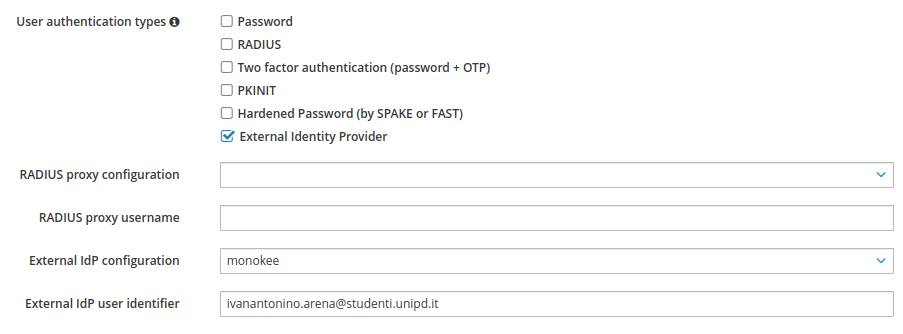
\includegraphics[width=\columnwidth]{appendici/ipa-user} 
  \caption{Setup utente FreeIPA}
\end{figure}



\hypertarget{autenticazione-via-cli}{%
\subsubsection{Autenticazione via CLI}\label{autenticazione-via-cli}}
A questo punto è tutto pronto per autenticare l'utente creato sulla
macchina con Monokee. Bisogna accedere alla macchina con un utente
locale e lanciare i seguenti comandi per richiedere un ticket Kerberos
anonimo ed utilizzare il canale FAST per autenticarsi con l'utente che
si è creato precedentemente (in questo caso l'utente si chiama
\emph{monokee1}).

\begin{verbatim}
kinit -n -c ./fast.ccache
kinit -T ./fast.ccache monokee1
\end{verbatim}

Lanciato il secondo comando apparirà un link alla schermata di login di
Monokee e ad autenticazione avvenuta basterà tornare al terminale e
premere \emph{Invio}. Per verificare l'avvenuta autenticazione occorre
lanciare il comando \texttt{klist} e controllare che il \emph{Default
principal} corrisponda all'utente desiderato e che il ticket sia valido.

\begin{figure}[!h] 
  \centering 
  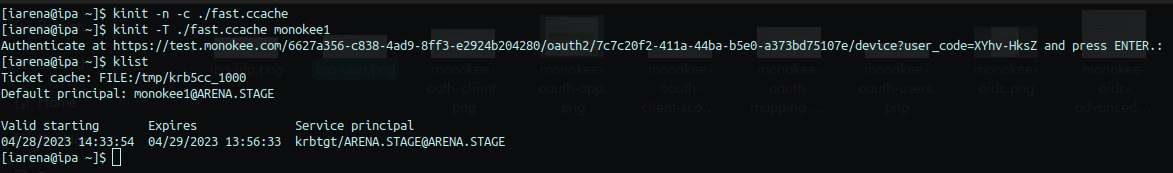
\includegraphics[width=\columnwidth]{appendici/ipa-cli} 
  \caption{Monokee SSO da CLI}
\end{figure}


\hypertarget{problemi}{%
\subsection{Problemi}\label{problemi}}

Di seguito elencati alcuni dei problemi rilevati.

\begin{itemize}
\item
  Facendo SSH su una macchina con un utente per il quale si è
  configurata l'autenticazione tramite Monokee, quindi non presente
  localmente ma gestito da FreeIPA, verrà chiesta la password, che non
  esiste per l'utente FreeIPA, perciò sarà impossibile accedere.
\item
  Potrebbe capitare che ci siano delle differenze tra i file di cache
  della macchina e quelli del server e che, quando si tenta l'accesso
  con \texttt{kinit} si riceva il seguente messaggio di errore:
  \texttt{ipa:\ ERROR:\ No\ valid\ Negotiate\ header\ in\ server\ response}.
  In tal caso un riavvio della macchina virtuale e della macchina dalla
  quale si sta facendo SSH dovrebbe risolvere.
\end{itemize}


